\documentclass[10pt]{article}
\usepackage[top=1cm, bottom=1cm, left=1cm, right=1cm]{geometry}
\usepackage{graphicx}
\usepackage{multicol}
\usepackage[colorlinks=true]{hyperref}
\usepackage{verbatim}
\usepackage{enumerate}
\usepackage{wrapfig}

\title{Wesnoth UMC Development \\ User's Manual}
\author{Timotei Dolean - \href{mailto:timotei21@gmail.com}{timotei21@gmail.com}}

\begin{document}

\maketitle

\tableofcontents
\setcounter{tocdepth}{3}
\newpage

\newcounter{cnt}
\newcommand{\icnt}{ \stepcounter{cnt} \thecnt }

\section{Foreword}
\begin{multicols}{2}
  \begin{center}
    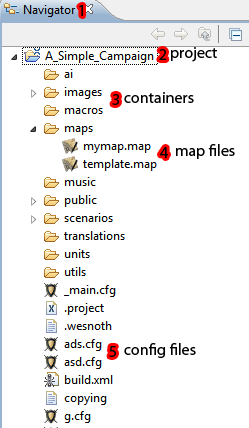
\includegraphics[scale=0.6]{definitions.png}
  \end{center}
The plugin has its homepage at: \url{http://eclipse.wesnoth.org/} \\

Through this readme the following terms with the specified meaning will be used:
\begin{enumerate}
\item Navigator / Project Explorer / Package Explorer - an Eclipse view that shows the projects in the workspace
\item Project - a directory on the harddrive that is represented as a top directory in the navigator.
\item Container - this is a directory or a project. Basically it can contain any file or directory children.
\end{enumerate}

The following image will highlight the terms used: 1 - Navigator, 2 - Project, 3 - Containers, 4 - Map files, 5 - Config files that contain WML code
\end{multicols}

\section{Prerequisites}
A quick list before getting into details:
\begin{enumerate}
\item Java 6
\item Python 2.x
\item Wesnoth 1.9.x, trunk or newer
\item Eclipse 3.7 ( Indigo ) or newer (Only for the Eclipse Version)
\end{enumerate}

Now for getting all those items:
\begin{enumerate}
\item The plugin runs on the following platforms: Windows 32/64 bit, Linux 32/64 bit and Mac OS X 64bit. Note that \textbf{Mac OS X 32 bit} is \textbf{not supported}. If you want to know why, please consult the Frequently Asked Questions section.
\item Download and install Oracle/Sun's Java Version 6 (Java SE6): \href{http://java.sun.com/javase/downloads/widget/jdk6.jsp}{Download JDK}

\textit{Note:} The plugin uses Java SE6, thus older versions (like 1.4 or 1.5) don't work with it.\\
\textit{Note:} Please double check the java installed on your system. On some machines there is the OpenJDK or other Java versions. Just use Oracle/Sun's so there will be no problems.

\item Download and install Python 2.x:
 \begin{enumerate}
   \item \textbf{Windows:} Download and install it from here: \href{http://python.org/download/}{Download Python} , selecting a 2.x version
   \item \textbf{Linux:} Use the distribution's package manager for installing it.
   \item \textbf{Mac:} Download and install it from here: \href{http://python.org/download/}{Download Python} , selecting a 2.x version
   \item For other operating systems, check the guide over here: \href{http://wiki.python.org/moin/BeginnersGuide/Download}{Python download and install}
  \end{enumerate}
 \textit{Note:} Please ensure you install the 2.x version. Version 3.x is \textbf{not} yet supported by the Wesnoth's WML Tools.

\item You will need to have a wesnoth version 1.9.x, trunk or newer, in order for the plugin's features to correctly work.

\item \textit{Note:} The following 2 steps are only neccessary if you will use the Eclipse version of the plugin.

\item Download ``Eclipse" (The download links are in the right. Please ensure you are downloading at least the \textbf{3.5} version, otherwise the plugin will not work. Also, \textbf{don't} download a \textbf{64 bit version} unless you are sure you have Java JDK on 64 bit. If you are unsure, select the 32 bit version):   \href{http://www.eclipse.org/downloads/packages/eclipse-classic-37/indigor}{Download Eclipse Classic}

\item Extract the downloaded archive in a known location and launch the executable (eclipse / eclipse.exe)

\end{enumerate}

\section{Installing the plugin}

\subsection{Eclipse version}
The Eclipse version, like the name says, needs a working Eclipse environment.

\begin{enumerate}
\item After launching Eclipse, go to the ``Help'' menu - Install new Software. Then, check the checkbox ``Contact all update sites during install to find required software" (it can be found in the bottom of the page).

\begin{center}
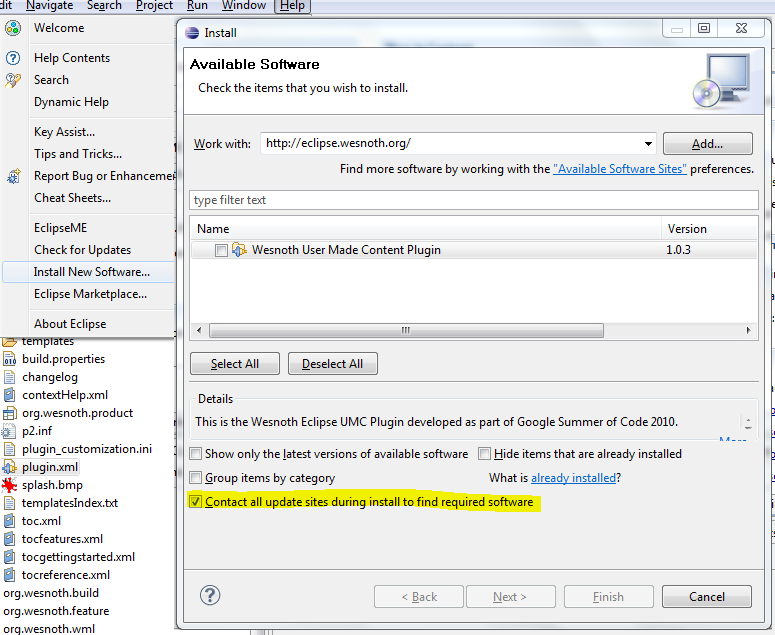
\includegraphics[scale=0.7]{install_new_software.png}
\end{center}

\item Insert the link \textbf{http://eclipse.wesnoth.org/updates} in the textbox in the top and press Enter. The list will be populated with some items.
\item Select the single item ``Wesnoth User Made Content Plugin" and press finish.

\textit{Note:} If you are prompted for any license agreements or certificates press Yes on all (if you agree).\\
\textit{Note:} After the plugin has installed, press ``Restart workbench now" when you are prompted.
\item Now the plugin is ready to be used.
\end{enumerate}

\subsection{Standalone version}
The standalone version of the plugin, does not need any Eclipse ``thingy". Just fulfil the prerequisites and you're ready to go. The standalone version is currently available as zip archives for major OSes (Windows, Mac OS X and Linux) and Architectures (x86 and x64). To use the standalone version follow the following steps:

\begin{enumerate}
  \item Go to \href{http://eclipse.wesnoth.org/doc\_howto.html}{http://eclipse.wesnoth.org/doc\_howto.html}
  \item Download the version appropiate to your OS and architecture.
  \item Extract the downloaded archive and launch eclipse executable (Eclipse.App / Eclipse.exe / Eclipse ).
\end{enumerate}

\section{Features}

The plugin has the following list of abilities (not exhaustive):
\begin{itemize}
  \item Easily creation of UMC Addons
  \item Quick ``Writing" of WML code by using WML Wizards, by focusing on the content
  \item Integrated launch of the Game or Map Editor
  \item Integrated launch of the WML tools on individual projects/files
  \item Support for multiple Wesnoth versions
  \item Integrated powerful WML Editor with autocomplete, go to macro definition, etc
\end{itemize}

\section{Using the plugin}
After you have started the plugin, you can use its features.

But before of all, you must setup your environment, so it knows where your wesnoth game is located. By default, after you have launched the plugin for the first time, you will be greeted with a small assistant that will help you ``setup the workspace". The preferences page for the plugin will pop up and you must fill all fields, so the plugin will work as intended. After you completed the fields, press \textbf{OK}. Then the plugin will create for convenience (i.e. if you want) wesnoth projects for each directory in your \textbf{useraddons/data/add-ons} directory. The working directory is the directory that contains the data, images, manual, sounds directories of Wesnoth.

If there were no errors a message window will open saying: \textbf{Workspace was setup successfully}.

\subsection{Wesnoth installations}
The plugin supports working with multiple installations ( we'll call them ``installs" ). The installs can be setup from the Preferences panel. An installation is called valid if:
\begin{itemize}
  \item It is defined in the Installs page
  \item It has set all paths and they point to existing objects (currently the following paths can be set: wesnoth working directory, wesnoth executable path, wesnoth user addons directory and wesnoth wml tools path)
\end{itemize}

The Installs Preferences Page will list all currently saved installs. You can view, edit, remove or set as default a specific installation.( \textit{Note:} You cannot modify the name of the install after creation. For that, you need to delete and add it again with another name.) The installs have also attached a Wesnoth version to them. This is for now, just for informational purposes. It is not used effectively in others area than the Preferences page.

All installs have in common the same python path. That means, each installation points to the same, current Python path set.

A default installation, is used at times like:
\begin{itemize}
  \item A new project is created
  \item A project uses a previous existing install, which is no more valid
\end{itemize}
The first created install ever will become automatically default. If a default installation is deleted and there are another installs, one of them will be selected as the new default.

After the user has configured the installs, he can use them on a per-project basis. Each project has a properties page ( Right click on project -$>$ Properties -$>$ Wesnoth Project ). There the user can configure project specific settings, including the install used in the context of that project.

\subsection{Wizards}
There are some wizards available in the plugin, that will create either projects or config files, based on the specified input. This wizards are available by going to the ``File" menu - New, and from that list selecting one of the Wesnoth wizards.

There are 3 wizards categories:
\begin{enumerate}
\item Project wizards - ``Empty project" and ``Campaign" wizards create new projects in the workspace. The former will create a basic addon directory structure. The latter will create a campaign and its directory structure.
\item File wizards - ``Wesnoth config file", ``Scenario", ``Era" and ``Faction" wizards create a new file in a selected container.
\item Wizard launcher - This is a special wizard. It takes a wml tag as input, and generate subsequent needed tags and key inputs. This is generated based on the wml schema, so if the schema is incomplete some tags won't be available. This wizard can create a new file or copy the resulted WML into the current edited file.
\end{enumerate}

\subsection{Menus}
There are currently 2 types of menus: the context menus for different file/container types and the main menu. For a better distinction the menus have the wenoth icon near each item.

\begin{description}
\item{\textbf{Project context menu}} - right click on the projects created with the plugin

   \textit{Wesnoth project report} - will show a simple report with the numer of maps, scenarios and units.\\
   \textit{Open campaign in game} - will start the current project's campaign (if any) in wesnoth. For this to work, you must have a ``\_main.cfg" file defined, and a campaign in it.\\
   \textit{Upload addon} - will upload the specified directory on the wesnoth addon server. The status will be outputed to the console.\\
   \textit{Regenerate build files} - recreates the ``build.xml" file. That is used if the current project is one relative to useraddons\\
   \textit{Builders} - utilities for adding/removing the wesnoth/xtext builders. Don't use them until you know what you are doing.

\item{\textbf{Container context menus}} - right click on any container

    \textit{WML Tools} - provides some options for using the wmltools with the specified project.

\item{\textbf{``maps" folder context menu}} - right click on the ``maps" directory

   \textit{Import map} - Shows a file selection window that will ley you select a .map file that will be copied in your maps directory.

\item{\textbf{.cfg files context menu}} - right click on any .cfg file

   \textit{Open scenario in game} - opens the selected file's scenario (if it contains one) in wesnoth.\\
   \textit{WML Tools} - provides some options for using the wmltools with the specified file. (e.g. run wmllint against the file and see the output in the console) \\
   \textit{Preprocessor} - provides ways of preprocessing and showing the result in an editor inside eclipse.

\item{\textbf{.map files context menu}} - right click on any .map file

   \textit{Open map in editor} - will open the selected map in the wesnoth map editor.

\item{\textbf{Editor context menu}} - right click in the editor
   \textit{Validate} - will validate the entire file (this is an expensive action)

\item{\textbf{Main menu}} - This is a menu near the ``Window" menu bar

   \textit{Open editor} - Will open the game editor with a blank map.\\
   \textit{Open game} - Will open the game.\\
   \textit{Import map} - It will import a map in selected container.\\
   \textit{Open editor} - Open the selected map in the game editor.\\
   \textit{Setup workspace} - Will setup the workspace if it's not setup. This will open the preferences page if any preferences is missing, and then it will create the wesnoth project for mainline and user addons directories if you want.\\
   \textit{Open plugin's preferences} - Opens the plugin preferences page.\\
\end{description}

\section{WML Editor}
The plugin contains a full-fledged WML Editor. It recognizes the .cfg files and opens them in the WML Editor by default. The Editor supports UTF-8 files not just ASCII ones. The editor is one of the most important features of the plugin.

\textit{Note:} Albeit the editor can open external files ( that is, outside the workspace ), all the cool features that come with the editor, will not be available until the file belongs to a project.

\subsection{Content assist}
At any time, when writing WML Code, one could activate the content assist by the \textbf{CTRL + SPACE} shortcut. A small inline popup will open showing suggestions on what to complete. Currently the plugin can auto complete:
\begin{itemize}
  \item Scenario ids
  \item WML Tags
  \item WML Keys
  \item WML Macros
\end{itemize}

Each item has a little icon to help the user distinguish between suggestions types.

\subsection{WML macros}
One can view the definition of a WML macro, by hovering / going with the caret over the call, and pressing \textbf{F2}. A small popup will open showing the macros' definition. Alternatively, Pressing \textbf{F3}, will open the macro's definition file, so you can modify it or inspect related macros.

\section{Use cases}
\subsection{Import an already existing wesnoth addon into the plugin}
For this you need just 2 single steps:
\begin{enumerate}
\item Open eclipse. Click the ``New" main menu bar - Project. Select the ``Empty project" from ``Wesnoth" category.
\item Enter the name of the project. Uncheck ``Use default location", and press ``Browse...". Navigate to the addon's directory and then continue the wizard as necessary.
\end{enumerate}

\subsection{Updating the plugin}
The plugin, due to Eclipse's architecture, can be updated very simple. At any time, the user can check for new updates, by going to the menu: Help-$>$ Check for Updates. If there are any new versions released, they will get downloaded and applied. This way you'll need to download just the bits updated, not the whole eclipse or standalone version.

\section{Frequently Asked Questions}

\subsection{What is this plugin all about?}
The plugin is in fact something like a WML IDE ( \href{http://en.wikipedia.org/wiki/Integrated_development_environment}{Wikipedia - IDE}). Basically it offers you some features that greatly help anybody who makes User Made Content in WML.

\begin{description}
\item - It has wizards for new campaigns, scenarios, factions, eras, and everything else you might think of. You just complete the needed values and it generates the wml (with nice indentation).
\item - It has front-ends for launching wmltools (like wmllint, wmlscope, wmlindent on files/directories), the wesnoth game, and the map editor.
\item - It has a specialized WML editor that has syntax highlighting, tag folding and outline, autocompletion, navigation to macro definitions and so on.
\item - It has integrated addon management features that allow to upload or download arbitrary addons.
\end{description}

\subsection{The IDE doesn't start anymore after update}
If you have just used the auto-update mechanism, and after the restart the IDE doesn't start anymore, then you can use a simple script to fix it. Just go to the download page (\url{http://eclipse.wesnoth.org/download.html}) and download the "Post-Update fix" script for your Operating System and execute it. Place it on the same level with the UMC IDE binary (wesnoth\_umc\_dev), and run it. Now the IDE should start fine.

\subsection{Where can I submit any bugs found?}
Go over to Wesnoth's bug tracker: \href{https://gna.org/bugs/?func=additem&group=wesnoth&bug_group_id=116}{Add new bug}. Please be as specific as possible. Also, if you have any logs, please attach them - refer to the next FAQ Entry for ways of getting the logs.

\subsection{Where I can find the logs?}
If you encounter any errors during the usage of the plugin, the plugin logs them in the: \textbf{$<$your temporary directory$>$/wesnoth\_plugin/logs}.
That is usually on linux:\\
\indent \textbf{/tmp/wesnoth\_plugin/logs}\\
or on windows:\\
\indent \textbf{C:/Documents and settings/$<$your username$>$/Local Settings/Temp/wesnoth\_plugin/logs} \\
or\\
\indent \textbf{C:/Users/$<$your username$>$/Local Settings/Temp/wesnoth\_plugin/logs}

\subsection{Why Mac OS X 32 bit is not supported?}
Apple decided to manage itself the versions that can run on each Mac version. Thus the modern Java SE6 version - which is used by the plugin - is not available on 32 bit Macs but on 64 bit only. The 32 bit Macs have just Java SE5 version available. Trying to port the plugin to the ``outdated'' java version is not likely to be done, so please consider upgrading your OS.

\end{document}
